\documentclass[10pt,a4paper]{report}
\usepackage{graphicx}
\usepackage{amsmath}
\usepackage{fancyhdr}
\usepackage{cite}
\usepackage{framed}
\usepackage{a4wide}
\usepackage{float}
\usepackage{epsfig}
\usepackage{longtable}
\usepackage{enumerate}
\usepackage{afterpage}
\usepackage{multirow}
\usepackage{ragged2e}
\usepackage{gensymb}
\usepackage{amsfonts} 
\usepackage[left=1.5cm,top=0.5cm,right=1.5cm,bottom=0.5cm]{geometry}
\usepackage{setspace}           
\usepackage{float}
\usepackage{txfonts}
\usepackage{lipsum}
\usepackage{titlesec}
\usepackage{mathtools}
\DeclarePairedDelimiter{\abs}{\lvert}{\rvert}

\titlespacing\section{0pt}{12pt plus 4pt minus 2pt}{0pt plus 2pt minus 2pt}

\newcommand{\Usefont}[1]{\fontfamily{#1}\selectfont}

\usepackage{lscape} % for landscape tables
\renewcommand{\baselinestretch}{1.7} 

\usepackage{blindtext}
\usepackage{xpatch}
\usepackage{url}
\usepackage{leqno}
\usepackage{subcaption}

\linespread{1.5}
\usepackage[intoc, english]{nomencl}
\hyphenpenalty=5000
\tolerance=1000
\usepackage[nottoc]{tocbibind}

% ******* References config *********
\bibliographystyle{IEEEtran}   % On some TeX systems this works
%\bibliographystyle{ieeetr}      % While on others this works
							% Uncomment and test if your references don't cite
							% correctly
\renewcommand{\bibname}{References}


%*********************Figures*****************************
% Save all figures in the folder figures and include them in your 
% report using the command \includegraphics{figure-name}

\graphicspath{{figures/}}

% figure files can be in jpeg,jpg, png or pdf formats
%*******************************************************************


\begin{document}
	
	
%****The entries in this section are to be filled in by the student with appropriate values *************

% These values are used thoroughout the report 
% please fill in the appropriate values in the brackets {}

\gdef \title{Software Radio Fall 2023 Final Project Submission } % Project title
\gdef \author{Grant Brown}	 %student name
\gdef \dept{Electronics and Communication Engineering} %Department
\gdef \college{College of Engineering University of Utah} % Name of the College
\gdef \collegeplace{Salt Lake City, UT} % Location of the College
\gdef \studentA{Grant Brown} %Project batch member 1

\gdef \acadyear{2022 - 23} % Academic year
\gdef \month{December 2023} %Month of Report submission
\gdef \date{15-12-2023} %Date of signing the declaration

%*******************************************************************
% The font pages. The source tex files are there in the folder
%==================================coverpage.tex================================


\newenvironment{coverpage}
\thispagestyle{empty}
\begin{titlepage}
	\begin{center}
		{\Usefont{phv} \Large \bf \title \par}
		\vspace*{40pt}
		\large \em \Usefont{pzc}{ 
			A Project Report \par
			Submitted to the Professor Farhang}\\ [.15\baselineskip] \par
		\Usefont{ppl} {\bfseries  \degree}\\
		by\\
		\bf {\studentA}\\
		\vspace*{170pt}
		\centering
		\begin{figure}[h!]
			\centerline{
\includegraphics[scale=0.4]{figures/uofu_logo.png}}
		\end{figure}
		
		\vspace{\stretch{0.5}}
		\footnotesize{\bf DEPARTMENT OF ELECTRONICS AND COMMUNICATION ENGINEERING} \par
		\bf{COLLEGE OF ENGINEERING UNIVERSITY OF UTAH} \par
		\bf{\month}
	\end{center}		
\end{titlepage}	
 %Unless essential Do not edit this tex file



%%********************Body of the report**********
% Arabic numbering is used in the body of the report

\cleardoublepage
\setcounter{page}{1}
\pagenumbering{arabic}

%%********************Abstract**********
\section{Abstract}This work aims to develop the receiver portion of a software radio. It must take into account real-world issues encountered in software radio's, such as: carrier offset and timing phase offset due to crystal oscillator imperfections, as well as distortion introduced by various transmission mediums. In part I of the project the students must demodulate a undisturbed transmitted signal to baseband, acquire the optimal timing phase associated with the transmitted symbols, and extract the specified data. Part II and III of the project uses a channel that introduces distortion and the students must create a symbol-spaced equalizer and fractionally-spaced equalized to restore the Nyquist pulse. Part IV of the project introduces a carrier offset and phase drift into the transmitted data, requiring a carrier acquisition and tracking method to restore the symbols. Part V introduces a non-zero timing phase into the design and requires a symbol rate tracker to be implemented. Part VI is optional and utilizes an equalizer to perform tracking for carrier and timing phase offsets.

\vspace{-1.5em}
%%********************Section 1**********
\section{Section 1 - Introduction}As demonstrated in Figure~\ref{fig:comm-system}, transmission of signals in digital systems requires the use of: a transmitter, a channel, a receiver, and a equalizer. The job of the transmitter is to generate data symbols which are free of ISI that can be transmitted over the desired channel medium. This is accomplished by first encoding bits to data symbols, which are then passed to a Nyquist pulse shaper, and then modulated to the desired carrier frequency. The receiver must then demodulate the desired signal to the baseband, perform matched filtering to remove unwanted spectrum's, and then sample at the correct timing phase to obtain the transmitted symbols. Physical devices, such as crystal oscillators are used in this process which bring physical limits to the precision of demodulation and sampling precision. These limits bring arise two major issues. One issue is carrier offset, which occurs because the transmitted signal is frequency shifted by a carrier $cos(2\pi f_c + \Theta (t))$. To perform exact demodulation we must know the timing varying phase as well as the exact frequency at which the signal was modulated. Any inaccuracies can cause a slight frequency offset where out signal is not centered around 0 Hz and can result in a constellation rotation shown in Figure~\ref{fig:qpsk-rotate}. The other issue is timing recovery, which occurs because exactly recovering the signal after demodulation and filtering requires knowing the exact timings at which the Nyquist pulse was generated. These timings are referred to as the optimal timing phase. Any delta between the transmission timing phase and receiving timing phase can introduce ISI and disturb the Nyquist pulses.
In addition, desired channel mediums typically will introduce some level of distortion to the received signals spectrum through the addition of unwanted noise and auxiliary signals. It is imperative to remove this noise to restore the Nyquist pulse properties to ensure no ISI and correct symbol detection. Equalizers are designed to perform this deconvolution operation which restores the initial spectrum by correctly weighting the irregularities through trainable weights, similar to a Neural Network. 

The project explores these issues and potential solutions and implementations of these solutions through a 6-sectioned project. Most of the solutions introduced used in this project are pilot-aided or decision-directed methods. The transmitted signals consist of a preamble and payload as shown in Figure~\ref{fig:data_sequence}. The preamble consists of training symbols, which are called pilots, which are used to fine tune the receiver parameters to ensure the correct signals are received at the output of the subsystem. Part I focuses on the basics of recovering the timing phase from an ideal channel. Part II and III introduces channel irregulaitires into the design and requires symbol-spaced and fractionally-spaced equalizers to be implemented to restore the Nyquist pulses which removes ISI. Part IV explores carrier and phase offset and the rotation it causes in constellations. Part V requires students to utilize decision-directed methods to restore a drifting optimal timing phase. Part VI is optional and uses fractionally-spaced equalizers to perform all functions of the receiver.


%Part I implements the demodulation and timing recovery sequences in the receiver with a ideal channel.  We must determine where the preamble and payload sequences are located in the transmitted data to ensure correct detection of the signals. Part II explores channel distortion and allows us to implement a symbol-spaced equalizer to correctly undo the effects of the channel. Part III investigates the fractionally-spaced equalizer and how that can be utilized to undo the effects of the channel. Part IV investigates the carrier offset and phase offset situations that occur in communication systems and implement data-aided methods to correctly undo the frequency and phase offset. Part V introduces timing phase drift into the transmitted signals and requires us to use data-aided timing phase recovery mechanisms to correctly decode the transmitted signal. Part VI explores the use of fractionally spaced equalizers to perform phase, frequency, and timing offset of carriers.

\vspace{-1em}
%%********************Section 2**********
\section{Section 2 - Demodulation, Timing Acquisition, and Data Extraction}Part I loads the transmission data from an ideal channel. We may assume there is zero phase error and zero frequency offset. The transmitter performs modulation with a carrier wave of the form $cos(2\pi f_c t)$ where $f_c = 10^5 Hz$. This is determined by looking at the spectral content of the signal \textit{xRF1.mat} shown in Figure~\ref{fig:xbb_partI}, which mimics the shape of a square-root raised cosine frequency response around $f_c = 10^5 Hz$ as expected. To increase the received signal to have highest SNR ratio we utilize matched filtering. This match filter also operates as a low-pass filter which can remove all unwanted spectral content outside the baseband. The transmitter utilizes expansion to reduce the bandwidth of the transmitted signal, therefore we needed to decimate the signal at the correct timing phase to ensure the signal samples are correctly identified at the receiver. According to chapter 10, for pulses with less then 100\% excess bandwidth 3 spectral coefficients exist in the Fourier series of the ensemble power $E[y(t)^2]$ of the received signal. This leads to the closed-form solution for the ensemble average $E[y(\tau)^2] = {\rho}_0 + 2\abs{{\rho}_1} cos(\dfrac{2\pi}{T_b}\tau + \angle{{\rho}_1})$ where ${\rho}_0$ is the  component and ${\rho}_1$ is the first harmonic. The ensemble average is a dc-shifted sinusoid, Figure~\ref{fig:ensemble-power}, which was verified through the Matlab code. Since there is not channel distortion the optimal timing phase is the location of the peak of the sinusoidal graph. After some time to reach steady state, the peaks occur every 100 samples as expected due to expansion by 100. We find the first sample that correlates to the peaks which is sample 1 and then decimate by every 100 samples from there. To verify the preamble and payload are correctly deciphered we may look at the constellation shown in Figure~\ref{fig:parti-packet-constellation}. As shown we see that the data symbols are at the correct symbol mapping spots with the preamble being scattered around these four points.

It is stated that the preamble begins consists of four pilot sequences each of length 32. Therefore, if we cross-correlate the decimated baseband signal with the pilot sequence we obtain four peaks, as shown in Figure~\ref{fig:cross-corr-parti}. These peaks indicated strong correlation between the baseband signal and the pilot, which means that the two sequences are the same. Therefore if we know the pilot is N=32 symbols then 32 symbols after the last peak the payload begins. Since there is no channel distortion we should expect a perfect QPSK constellation as shown in Figure~\ref{fig:payload-constellation-parti}. Passing this data to the text file we are able to correctly decipher xRF1.mat which tells a joke.



\vspace{-1em}
%%********************Section 3**********
\section{Section 3 - Preamble Detection and Symbol-Spaced Equalizer}In Part II we explore how channel distortion can cause problems with ISI and how the use of equalizers can be used to solve non-ideal channel variance. To explore the mathematical model of the channels impulse response we note that the channel can be modeled as $c(t) = {\alpha}_i \delta (t-{\tau}_i)$ assuming a single-path channel. When using Nyquist pulses the equivalent baseband impulse response between the transmitter and receiver is $c_{BB}(t) = {\beta}_i p(t-{\tau}_i)$, where $p(t)$ is the convolution between the matched receiver and transmitter filters, and ${\beta}_i={\alpha}_i e^{-j2\pi f_c {\tau}_i}$ is a complex gain factor. If we assume that the delay incurred by the channel is insignificant the received signal at the demodulator gives $y(t) = \sum_{n=-\infty}^{\infty} s[n]c_{BB}(t -nT_b) + v(t)$ where $v(t)$ is noise added by a non-ideal channel. If we include the complex gain factor ${\beta}_i$ the complex baseband equivalent impulse response of the channel simplifies to $y(t) = {\beta}_i \sum_{n=-\infty}^{\infty} s[n]c_{BB}(t -nT_b) + v(t)$. In the absence of channel noise we have perfect Nyquist pulses spaced by $T_b$ at the output and sampling at these portions we can recover the transmitted symbols. When there is a significant delay in the channel or the channel has additive noise our assumptions fail and we must revert to the more general impulse response of $y(t) = \sum_{n=-\infty}^{\infty} s[n]c_{BB}(t -nT_b) + v(t)$. Here $c_{BB}(t)$ is not a perfect Nyquist pulse and ISI will occur. To restore the Nyquist pulse after the receiver we pass $y(t)$ through an equalizer, $w(t)$ whose cascade formation with the baseband channel impulse response, $c_{BB}(t) \star w(t)$, restores the Nyquist pulse shape to an acceptable level of ISI. The addition of multi-path channels follows the above discussion with an emphasis on the delay of the paths must be equal to ensure no ISI, otherwise an equalizer is needed.

In Part II we implement a symbol-spaced equalizer, as shown in Figure~\ref{fig:symbol-spaced}. By transmitting a sequence of pilot symbols we can utilize the cyclic equalization method shown in Figure~\ref{fig:symbol-cyclic}. The goal is to minimize the mean squared error between the equalized symbols and the pilot, $\abs{{e[i]}^2}$. To correctly utilize the cyclic equalizer we need to grab the preamble from the received signal. This can be done by performing an auto-correlation of the received and decimated signal. Theory says that when the transmitted signal is auto-correlated through the equation $r_{yy}(n, N+1) = \sum_{k=0}^{N} y[n-k]y^{\star}[n-N-1-k]$ we will obtain a flat top or constant auto-correlation, as shown in Figure~\ref{fig:auto-corr}, when transversing over the repeated pilot sequence. Grabbing any 32 symbol sequence from this flat section results in single period of the pilot sequence which is then used in the cyclic equalizer. The code to implement the cyclic equalizer is shown in Figure~\ref{fig:symbol-code}. The output of the weights may be shifted, as shown in Figure~\ref{fig:non-circ-weights}, due to an offset of where you grabbed the preamble and the at which symbol you start the pilot sequences. Since equalizer tap weights peak in the middle of the sequence and the channel impulse response also peaks in the middle we circularly shift the tap weights to be center aligned as shown in Figure~\ref{fig:circ-weights}. The effect of the equalizer can be shown through the a comparison of the constellation of the payload before and after equalization in Figure~\ref{fig:payload-equal-part2}.

Correct timing phase is critical for performance because the symbol spaced equalizer does not correct timing phase errors. Figure~\ref{fig:payload-equal-wrong-phase-part2} shows that the constellation of the decimated signal after equalization becomes less clear when compared to the optimal timing phase decimated sequence due to increased ISI. We will defer more detailed timing phase discussion until Part IV.

\vspace{-1em}
%%********************Section 4**********
\section{Section 4 - Fractionally Spaced Equalizer}Part III of the project requires us to implement a half-symbol spaced equalizer shown in Figure~\ref{fig:frac-equal}. Fractionally-spaced equalizers are more complex than symbol spaced since they operate at a higher data rate then the symbol spaced equalizers, however hold benefits that warrant the complexity increase. One key benefit that fractionally-spaced equalizers bring is that if they learning rate is fast enough they can deal with timing phase imperfections without the need for an explicit timing recovery method. The core theory behind this benefit is that timing phase imperfections are brought about by incorrect phase in spectral aliasing. When the data rate is high enough to avoid the spectral aliasing the timing phase will not depend on the phase of the overlap anymore as long as the fractionally-spaced equalizer is used correctly.

To correctly train the tap-weights we once again utilize the cyclic method shown in Figure~\ref{fig:cyclic-frac}. It is important to note that because of the expansion by L we have to grab L*32 samples of the preamble to get all symbols in the pilot. In the case of the half-symbol spaced equalizer L = 2 and M=1 where M is the decimation factor.To ensure the correct tap weights are associated with pilot symbols we must shift the preamble sequence by 2. Since the pilot is still 32 symbols we must perform this cyclic equalization over a two clock cycle span for each iteration. The general conclusions of the symbol-spaced equalizers are applicable to the fractionally spaced equalizer as well.

The eye pattern of the half-symbol spaced equalizer is shown for xRF3.mat in Figure~\ref{fig:payload-equal-part3}. As shown, the constellation becomes closer to ideal. Mathematically we can enumerate the performance of the equalizers by looking at the mean-square error of the two signals. 

\vspace{-1em}
%%********************Section 5**********
\section{Section 5 - Carrier Acquisition and Tracking}Part IV explores having carrier and phase offset in the receiver and channel and how that affects the constellations. The carrier $cos(2\pi f_c t + \Theta (t))$ is modulated by the data symbols at the transmitter. $\Theta (t)$ is a time varying phase that must be accounted for to avoid constellation rotation shown in Figure~\ref{fig:phase-rotate}. In addition to a time-varying phase the receiver must perform demodulation to move the transmitted data symbols back to baseband. If the carrier frequency and the demodulation sinusoid frequency are not exactly equal we will obtain resulting in the signal $y(t) = e^{j2\pi \Delta f_c t} \sum_{n=-\infty}^{\infty} s[n] h_0 (t-nT_b) + v(t)$ where $h_0(t)$ is the impulse response of the channel to the first data symbol. To obtain the ideal baseband signal of $y(t) = \sum_{n=-\infty}^{\infty} s[n] h_0 (t-nT_b) + v(t)$ we must determine the carrier offset $\Delta f_c$. Utilizing the pilot we can utilize the auto-correlation of $J = \sum_{n=N_1}^{N_2} y[n+N] y^{\star}[n]$. Expanding this signal we know $x[n] = x[n+N]$ which will give us $J=e^{j2\pi \Delta f_c t}\sum_{n=N_1}^{N_2}\abs{{x[n]}^2}$, which holds due to the uncorrelated nature of the noise $v(t)$ and the transmitted symbols $x[n]$. Solving for $\Delta f_c$ we get: $\Delta f_c = \dfrac{1}{2\pi NT_b}\angle{J}$. Note that the length of the periodic signal N determines the precision to what we can determine in carrier offset.

After the equalizer we may still be dealing with some residual phase offset of the signals. To alleviate this problem before detecting the final data we pass it through a data-directed phase tracking method shown in Figure~\ref{fig:phase-pll}. The theory behind this method is a predictive phase detector, which compares the slicer input and output. If the phase error is small enough then we can approximate the error as $\epsilon [n] = \dfrac{I\{\~s[n] \^s[n]\}}{R\{\~s[n] \^s[n]\}}$ where $\~s[n] \text{and} \^s[n]$ are the slicer inputs and outputs. This error is then passed to a tune-able loop filter which updates the phase for the next symbol.

Utilizing this procedure on xRF7.mat we can see the effect of the carrier phase offset in the constellation in Figure~\ref{fig:before-dd}. Applying the decision directed method to equalize the phase we get the constellation in Figure~\ref{fig:after-dd}, showing the need for the carrier phase offset removal.

\vspace{-1em}
%%********************Section 6**********
\section{Section 6 - Symbol Rate Tracking}In Part V of the project we must account for a time-varying timing phase which was inserted in the transmitted signal. In this case the optimal timing phase may not be every L samples from the initial transmitted symbol. This can arise due to non-ideal crystal oscillators and we therefore must determine at which decimation points we should grab the transmitted signal to extract the payload. In this part we must do an initial coarse timing recovery based on the theory discussed on Section II on the ensemble average power. Once that is done we find the maximum power peak and treat that as the beginning of decimation sequence on our transmitted packed. From this transmitted packet we use the previously discussed cross-correlation peak analysis, shown in Figure~\ref{fig:cross-corr-parti}. This allows us to detect the beginning of our payload. Once the payload has been detected we utilize a decision-directed timing recovery algorithm. The decision-directed method uses basic differential calculus to minimize the expectation of the error signal, $\xi = E[\abs{{e[n]}}]^2$ where $e[n] = s[n] - y(nT_b + \tau)$. Taking the derivative of the error to find a local minimum solution depending on our initialization point gives (unless function is convex) gives $\dfrac{d\epsilon}{d\tau} =  -2R\{(e^{\star}[n]\dfrac{dy(nT_b + \tau)}{d\tau})\}$. This gradient descent method then utilizes an approximation of this derivative to slowly move towards the optimal phase in each iteration.

Utilizing this algorithm on xRF9.mat shows the need to timing phase restoration. Without timing phase restoration, the QPSK constellation is of the form in Figure~\ref{fig:no-dd}. When timing phase and slicing is applied to latch to the closest symbol in the desired constellation our QPSK constellation is of the form in Figure~\ref{fig:with-dd} with the correct text output.

\vspace{-1em}
%%********************Section 7**********
\section{Section 7 - Use of equalizer for tracking of carrier offset and timing phase}In a receiver three functions operate concurrently: timing recovery, carrier recovery, and channel equalization. If the channel equalizer tap-weight adaptation algorithm is fast enough one may automatically compensate for an residual carrier offset $\Delta f_c$. However, if the carrier offset it too large then the channel equalizer cannot resolve this issue, therefore a coarse carrier recovery is needed at the beginning. As mentioned earlier, a fractionally-spaced equalizer can perform timing recovery, therefore the timing and carrier recovery blocks can be removed. This leads to a receiver system shown in Figure~\ref{fig:phase-pll} without the PLL, since the equalizer can solve for the phase rotation. The current implementation of the LMS algorithm has a convergence rate that is too low to track carrier offset issues with the constellation. The use of a faster adapting algorithm is needed for carrier offset tracking, such as the recursive least squares algorithm (RLS). The RLS algorithm projects the under-determined system to the solution with the smallest error vector within the systems vector space. The convergence characteristics shown in Figure~\ref{fig:lms-conv} and Figure~\ref{fig:rls-conv} show that the RLS convergence is an order of magnitude better then the LMS algorithm.

\vspace{-1em}
%%********************Section 6**********
\section{Conclusion}In this 6-part final project we have demonstrated understanding of the basics of software radio systems. We have explored the architectures for transmitter-channel-receiver systems, as well as common issues that may occur in these systems. We have equalized channel distortion using symbol and fractionally spaced equalizers. Results show that while symbol-spaced equalizers bare minimum complexity the advantages of the fractionally-spaced equalizer out-weight its added complexity. To solve non-ideal transmitter and receiver structures, we have utilized pilot and decision-directed methods to fix timing phase, constellation rotation, and carrier recovery. This has allowed for us to overcome common issues such as crystal oscillator imperfections to extract transmitted data at the output of the equalizer. 

Professor Fahrang, thank you for the great semester and patience as we learn the material. I greatly enjoyed the class and I am looking forward to learning more on this topic over time with your guidance.


%%********************Section 6**********
\newpage
\section{Figures}\begin{figure}[h!]
    \centering
    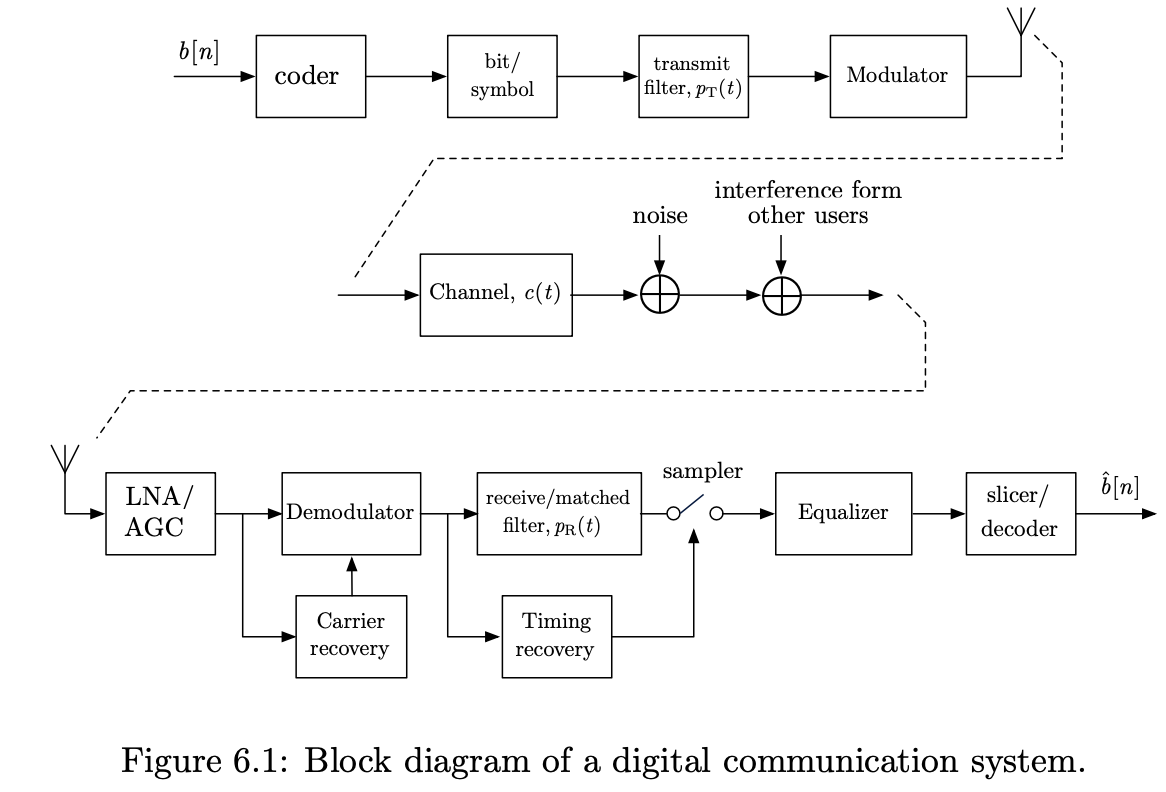
\includegraphics[scale=0.7]{figures/software_radio_system.png}
    \caption{Block Diagram of A Communications System}
    \label{fig:comm-system}
\end{figure}
\begin{figure}[h!]
    \centering
    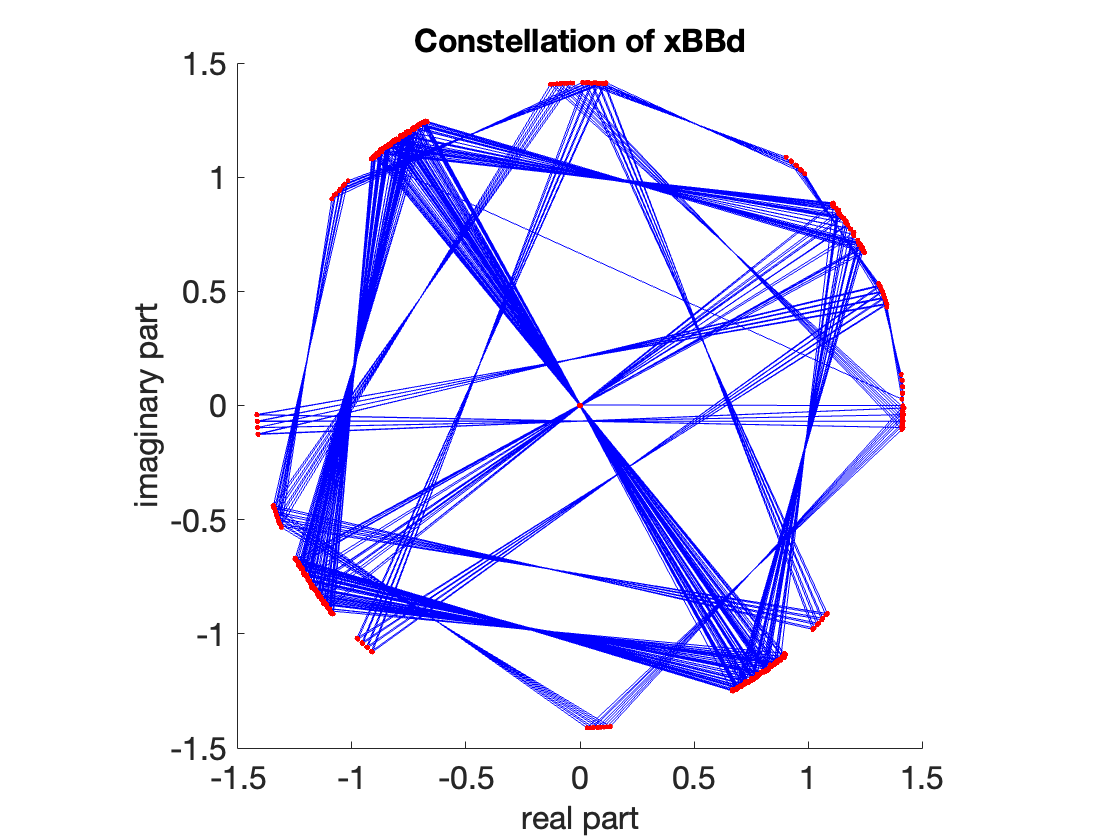
\includegraphics[scale=0.5]{figures/constellation_rotation.png}
    \caption{Result of Frequency Offset in QPSK Constellation}
    \label{fig:qpsk-rotate}
\end{figure}
\begin{figure}[h!]
    \centering
    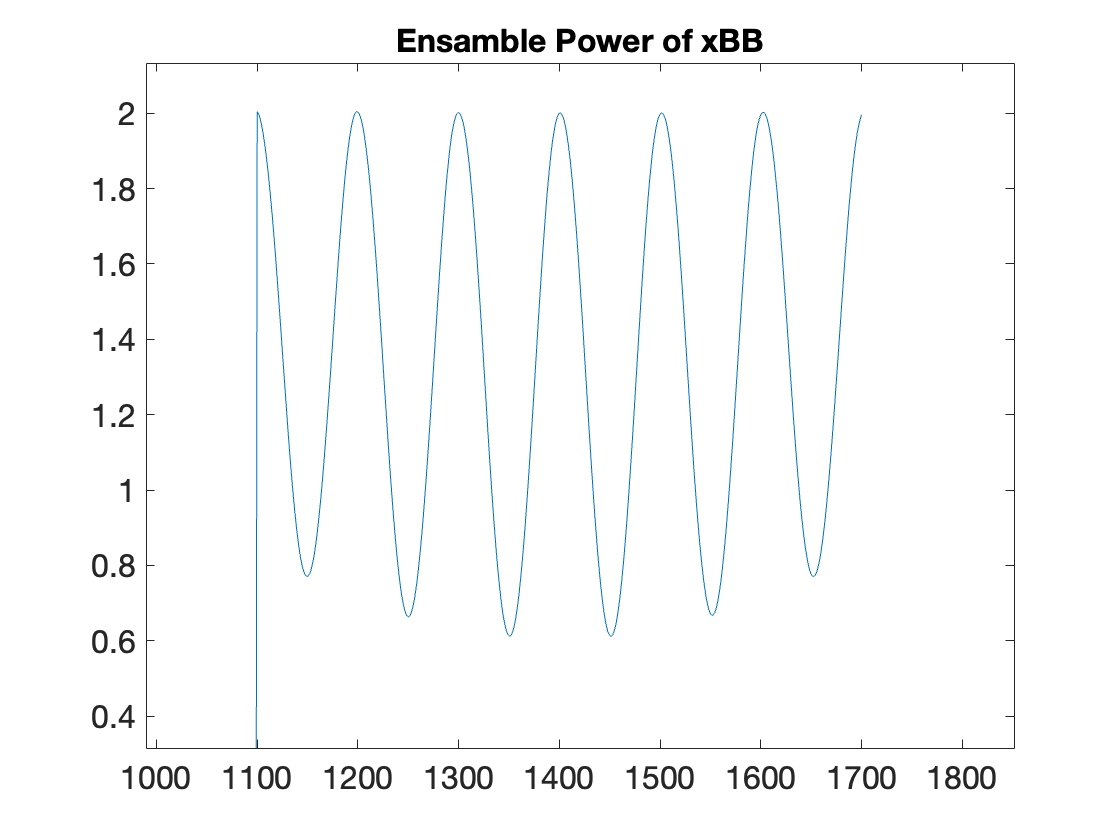
\includegraphics[scale=0.5]{figures/ensemble_power.png}
    \caption{Ensemble Power of xRF1.mat}
    \label{fig:ensemble-power}
\end{figure}
\begin{figure}[h!]
    \centering
    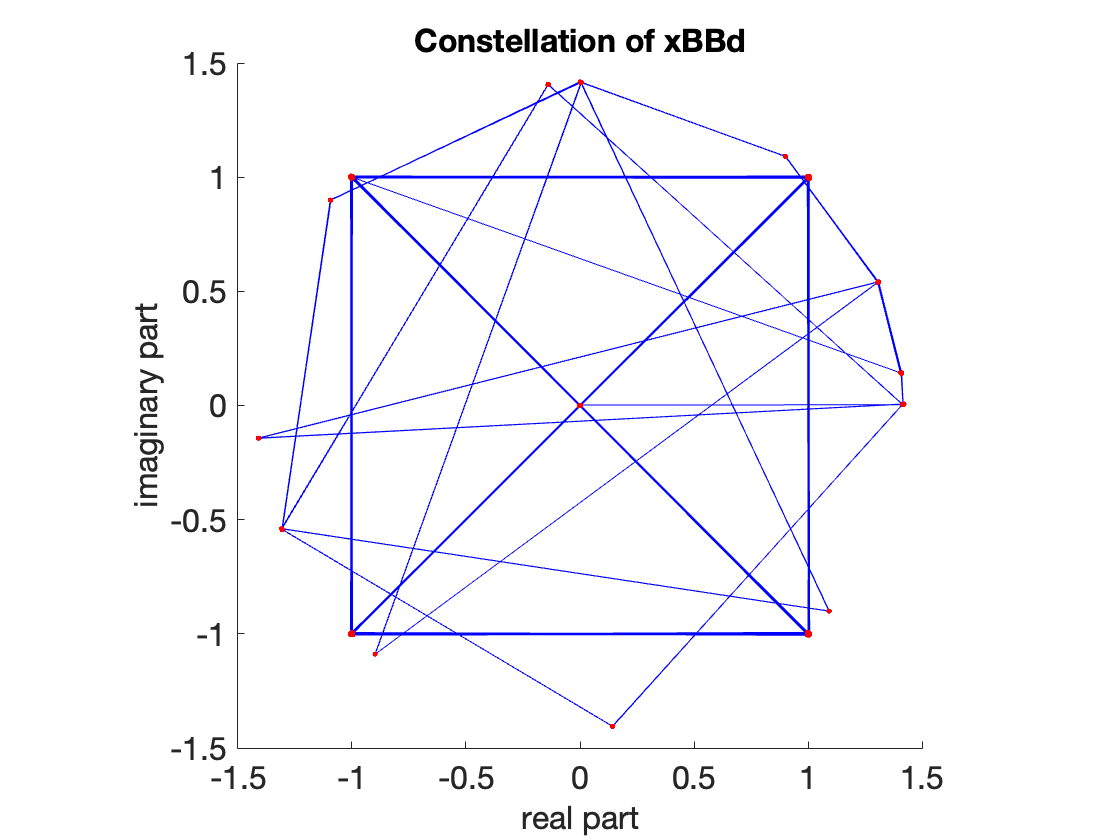
\includegraphics[scale=0.5]{figures/packet_qpsk_constellation.png}
    \caption{Packet QPSK Constellation of xRF1.mat}
    \label{fig:parti-packet-constellation}
\end{figure}
\begin{figure}[h!]
    \centering
    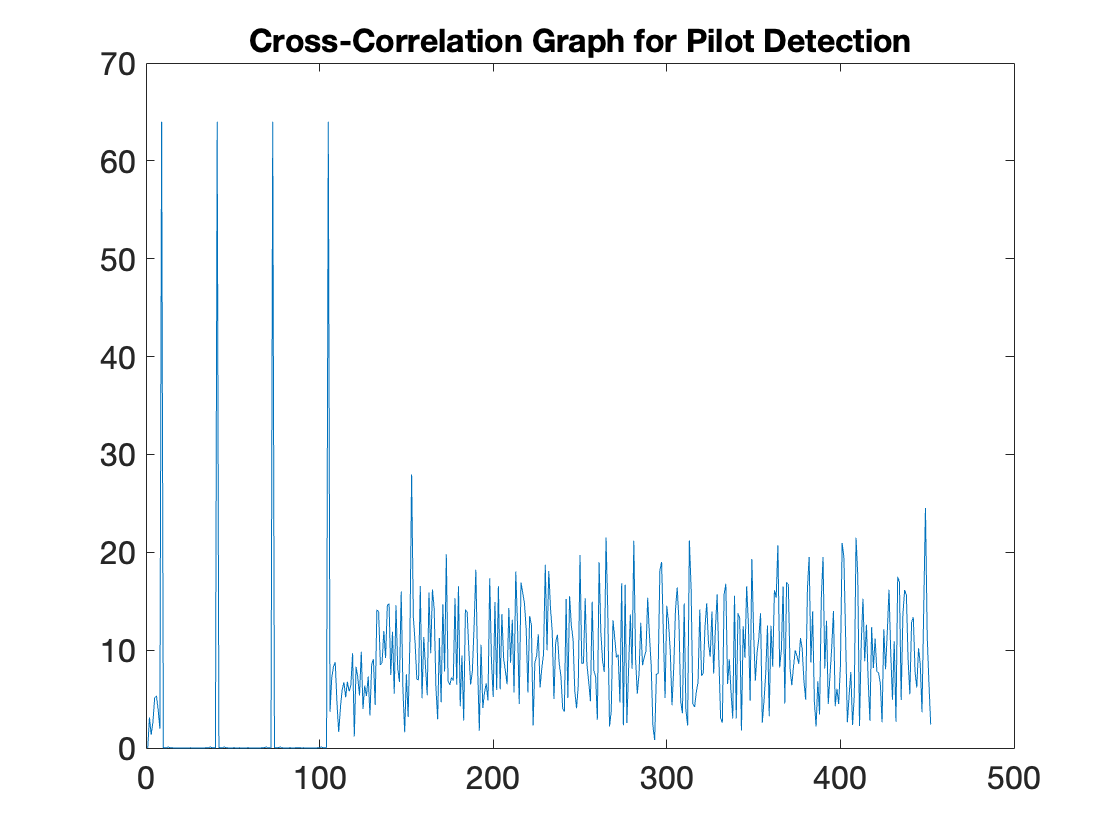
\includegraphics[scale=0.5]{figures/cross-correlation-parti.png}
    \caption{Cross-Correlation of Premable with Pilot of xRF1.mat}
    \label{fig:cross-corr-parti}
\end{figure}
\begin{figure}[h!]
    \centering
    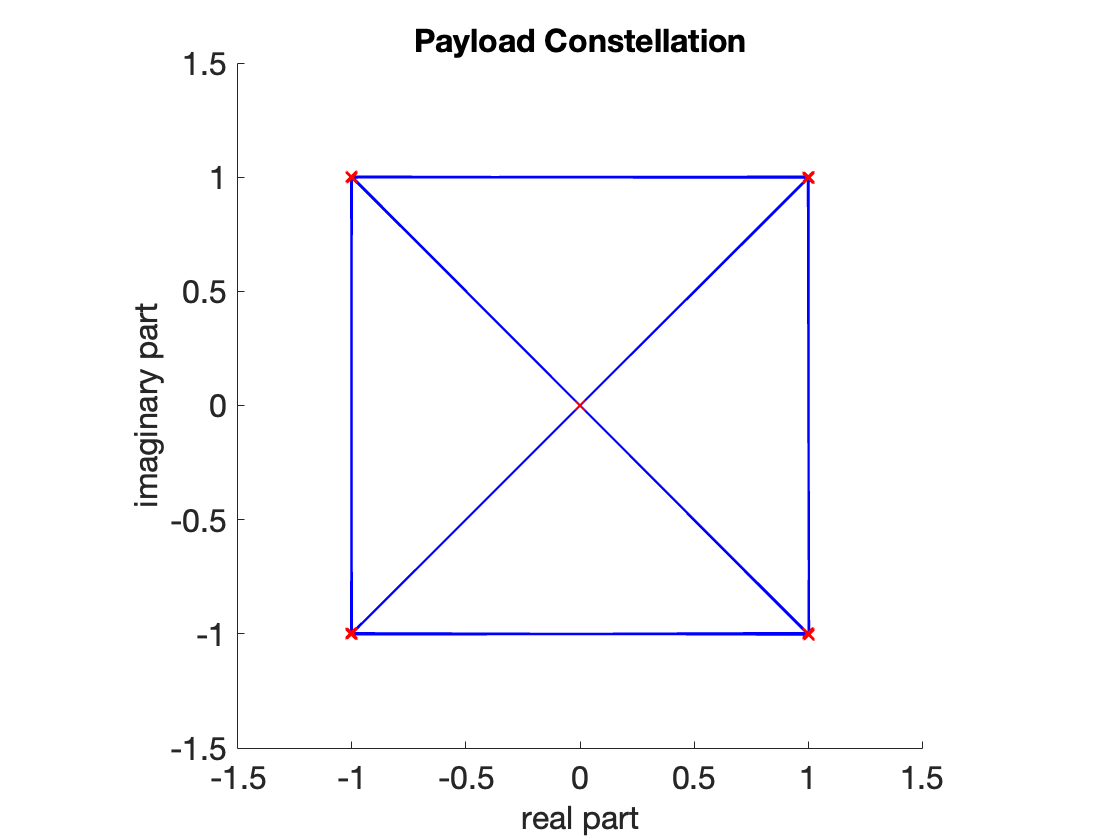
\includegraphics[scale=0.5]{figures/payload-constellation-parti.png}
    \caption{Payload QPSK Constellation of xRF1.mat}
    \label{fig:payload-constellation-parti}
\end{figure}
\begin{figure}[h!]
    \centering
    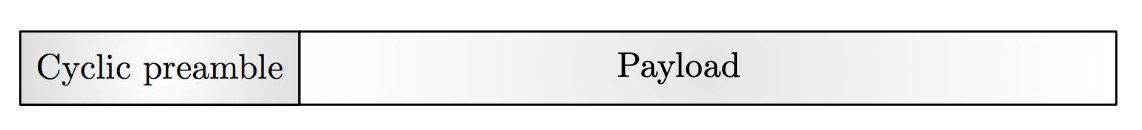
\includegraphics[scale=0.7]{figures/data_sequence.png}
    \caption{Structure of transmitted packets in project}
    \label{fig:data_sequence}
\end{figure}
\begin{figure}[h!]
    \centering
    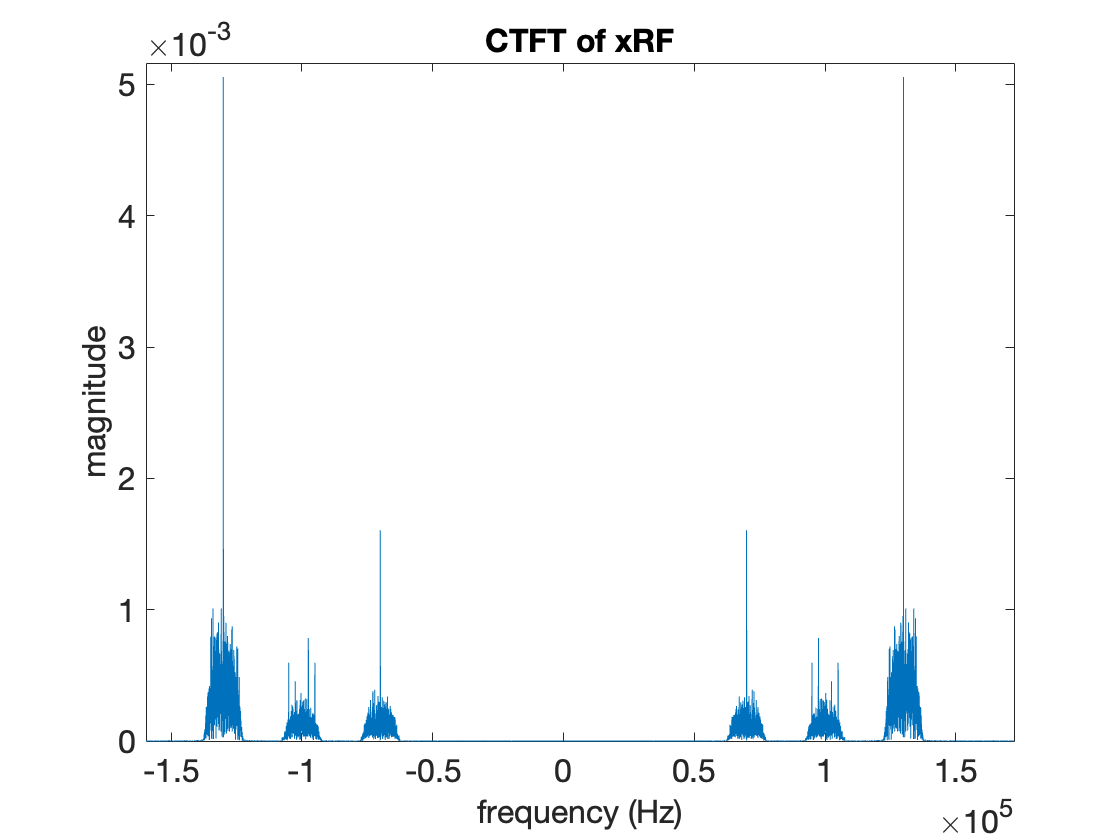
\includegraphics[scale=0.4]{figures/xRF1 spectrum.png}
    \caption{Spectrum of xBB signal in Part I}
    \label{fig:xbb_partI}
\end{figure}
\begin{figure}[h!]
    \centering
    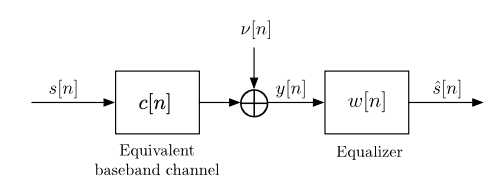
\includegraphics[scale=1.5]{figures/discrete_time_symbol_spaced.png}
    \caption{Discrete Time Symbol-Spaced Equalizer}
    \label{fig:symbol-spaced}
\end{figure}
\begin{figure}[h!]
    \centering
    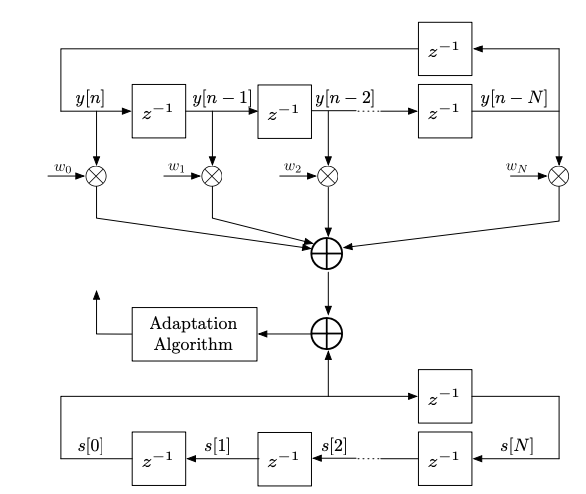
\includegraphics[scale=1]{figures/symbol_spaced_cyclic.png}
    \caption{Symbol-Spaced Cyclic Equalizer Training}
    \label{fig:symbol-cyclic}
\end{figure}
\begin{figure}[h!]
    \centering
    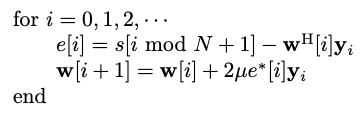
\includegraphics[scale=1]{figures/equalizer code.png}
    \caption{Cyclic Symbol-Spaced Equalizer Code}
    \label{fig:symbol-code}
\end{figure}
\begin{figure}[h!]
    \centering
    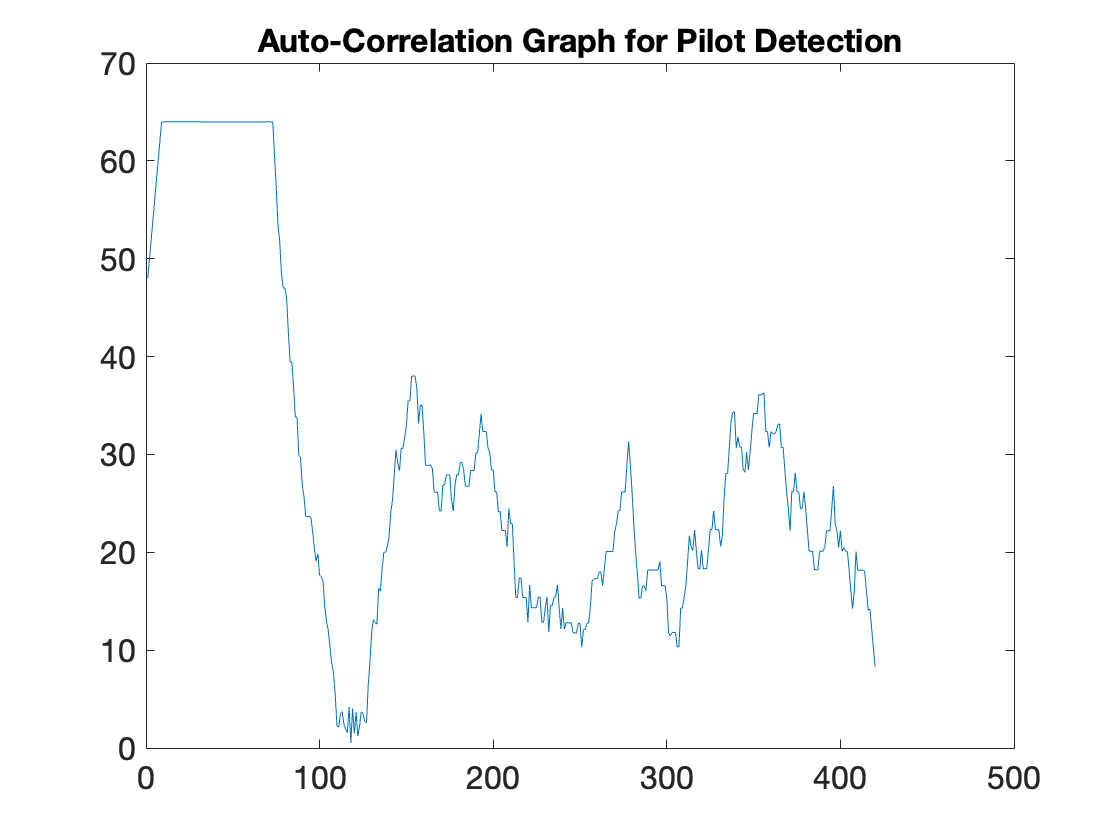
\includegraphics[scale=0.4]{figures/auto-correlation.png}
    \caption{Auto-correlation to Find Preamble on xRF1.mat}
    \label{fig:auto-corr}
\end{figure}
\begin{figure}[h!]
    \centering
    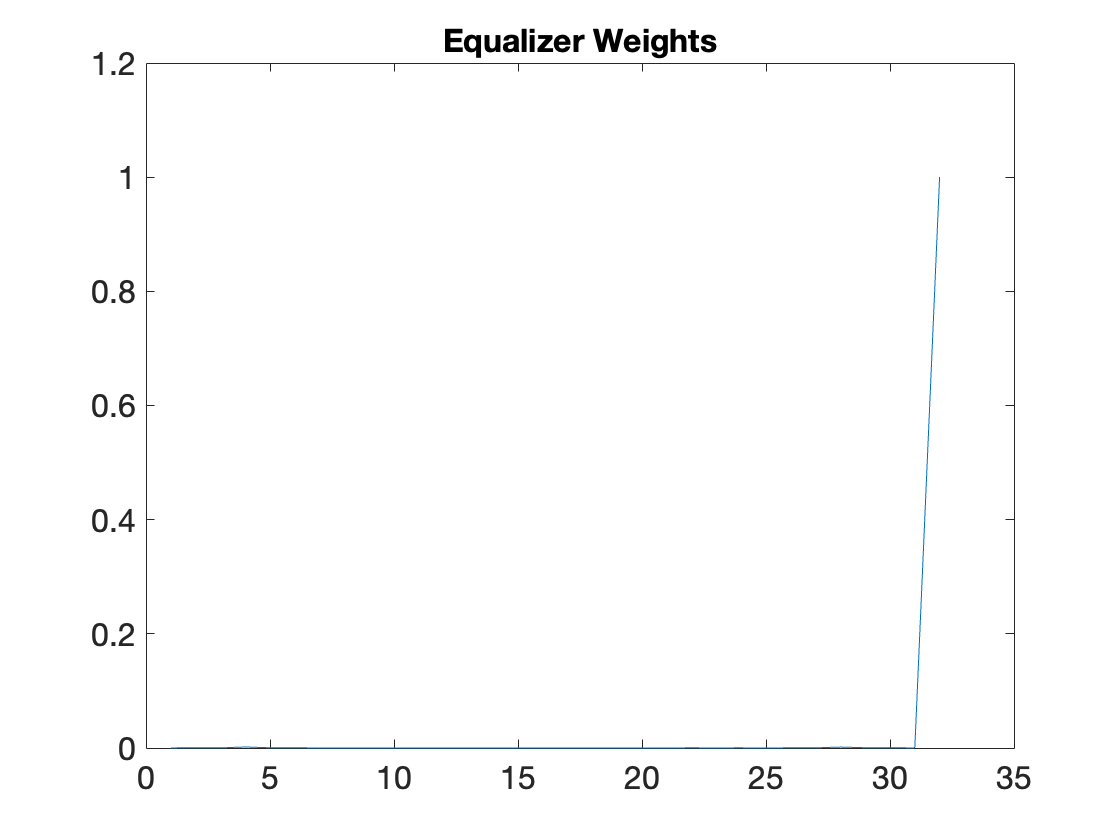
\includegraphics[scale=0.4]{figures/non_shifted_weights.png}
    \caption{Non-Shifted Tap-Weights of Symbol-Spaced Equalizer on xRF1.mat}
    \label{fig:non-circ-weights}
\end{figure}
\begin{figure}[h!]
    \centering
    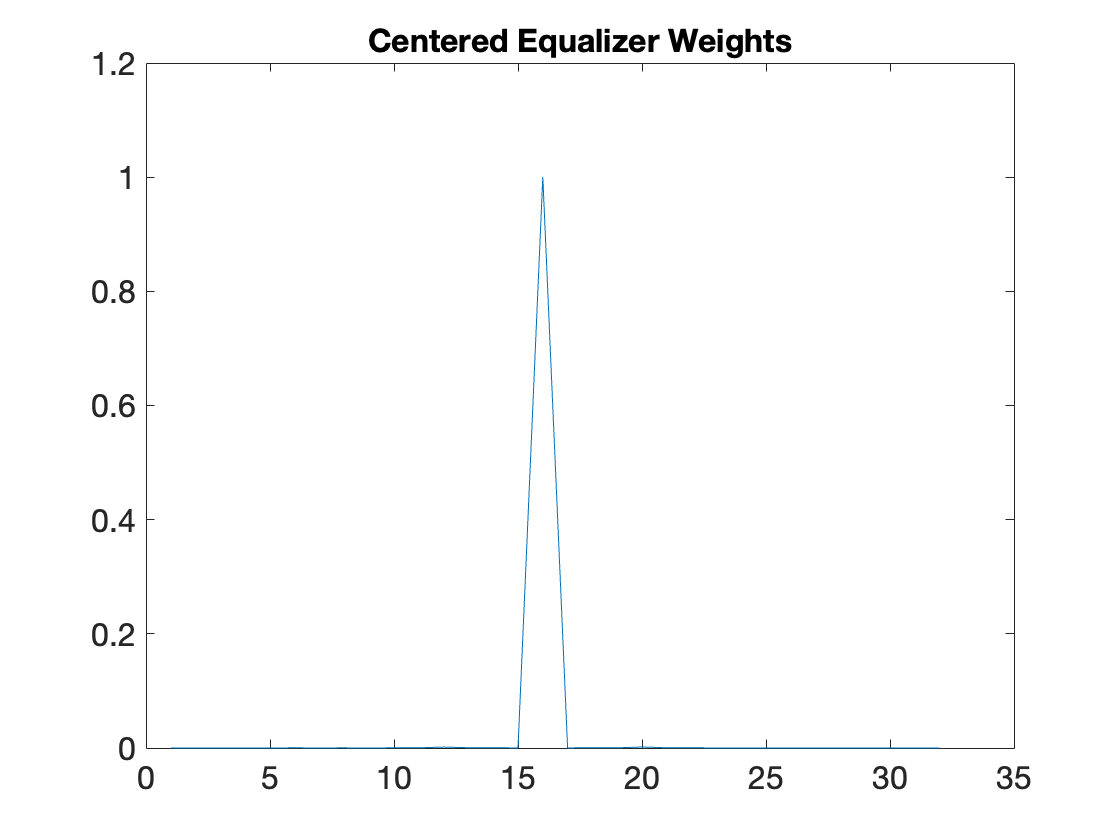
\includegraphics[scale=0.4]{figures/shifted_tap_weights.png}
    \caption{Shifted Tap-Weights of Symbol-Spaced Equalizer on xRF1.mat}
    \label{fig:circ-weights}
\end{figure}
\begin{figure}[h!]
    \centering
    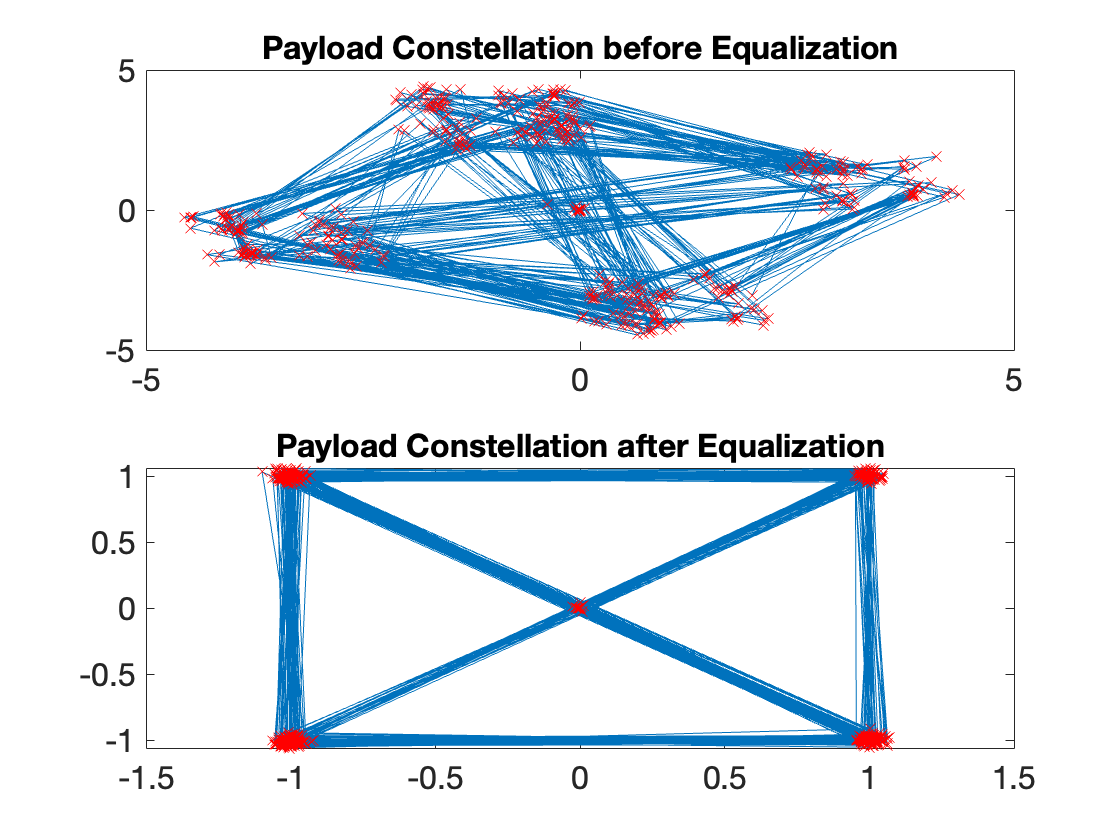
\includegraphics[scale=0.4]{figures/payload_equalization_part2.png}
    \caption{Payload Constellation of xRF3.mat before and after Symbol-Spaced Equalization}
    \label{fig:payload-equal-part2}
\end{figure}
\begin{figure}[h!]
    \centering
    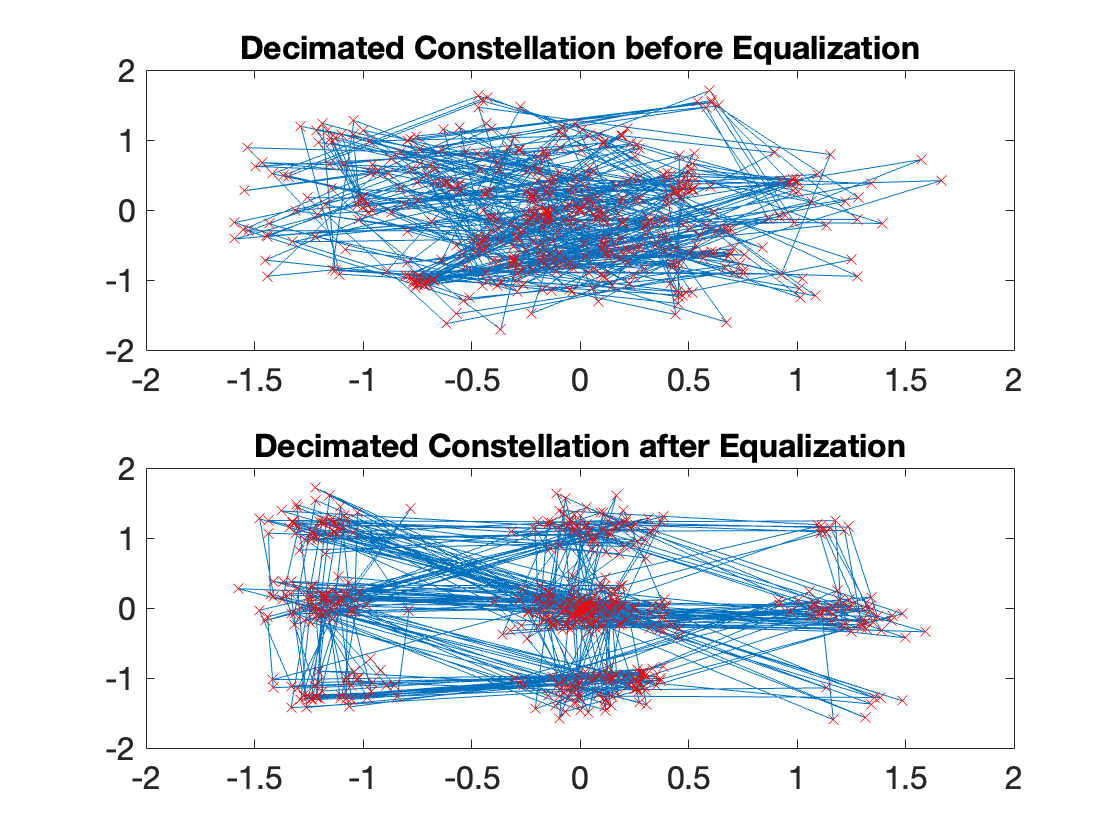
\includegraphics[scale=0.4]{figures/bad_timing_phase_part2.png}
    \caption{Payload Constellation of xRF5.mat before and after Symbol-Spaced Equalization with Wrong Timing Phase}
    \label{fig:payload-equal-wrong-phase-part2}
\end{figure}


\begin{figure}[h!]
    \centering
    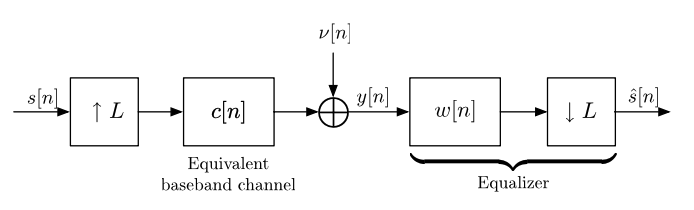
\includegraphics[scale=0.4]{figures/fractionally_spaced.png}
    \caption{Fractionally-Spaced Equalizer}
    \label{fig:frac-equal}
\end{figure}

\begin{figure}[h!]
    \centering
    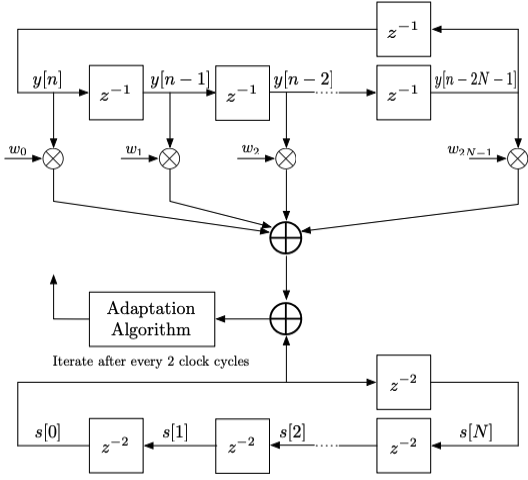
\includegraphics[scale=0.4]{figures/cyclic-frac.png}
    \caption{Fractionally-Spaced Cyclic Equalizer}
    \label{fig:cyclic-frac}
\end{figure}
\begin{figure}[h!]
    \centering
    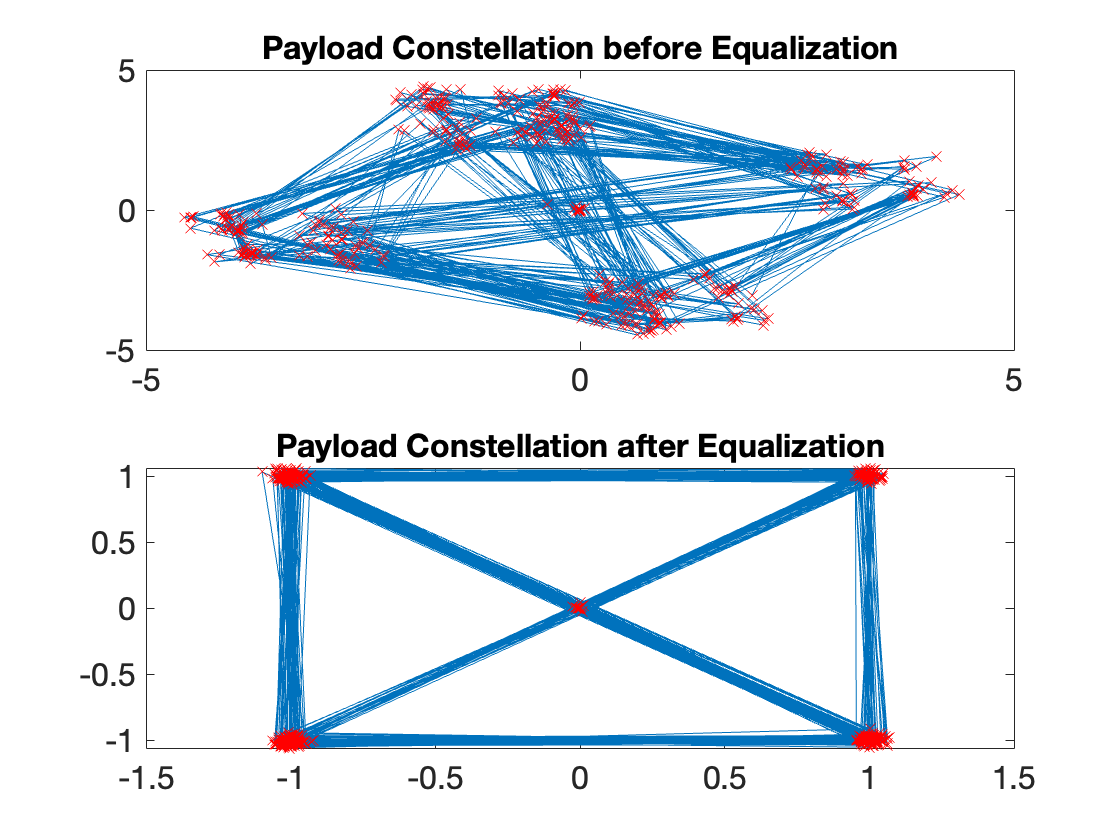
\includegraphics[scale=0.4]{figures/payload_constellation_part3.png}
    \caption{Payload Constellation of xRF3.mat before and after Half Symbol-Spaced Equalization}
    \label{fig:payload-equal-part3}
\end{figure}

\begin{figure}[h!]
    \centering
    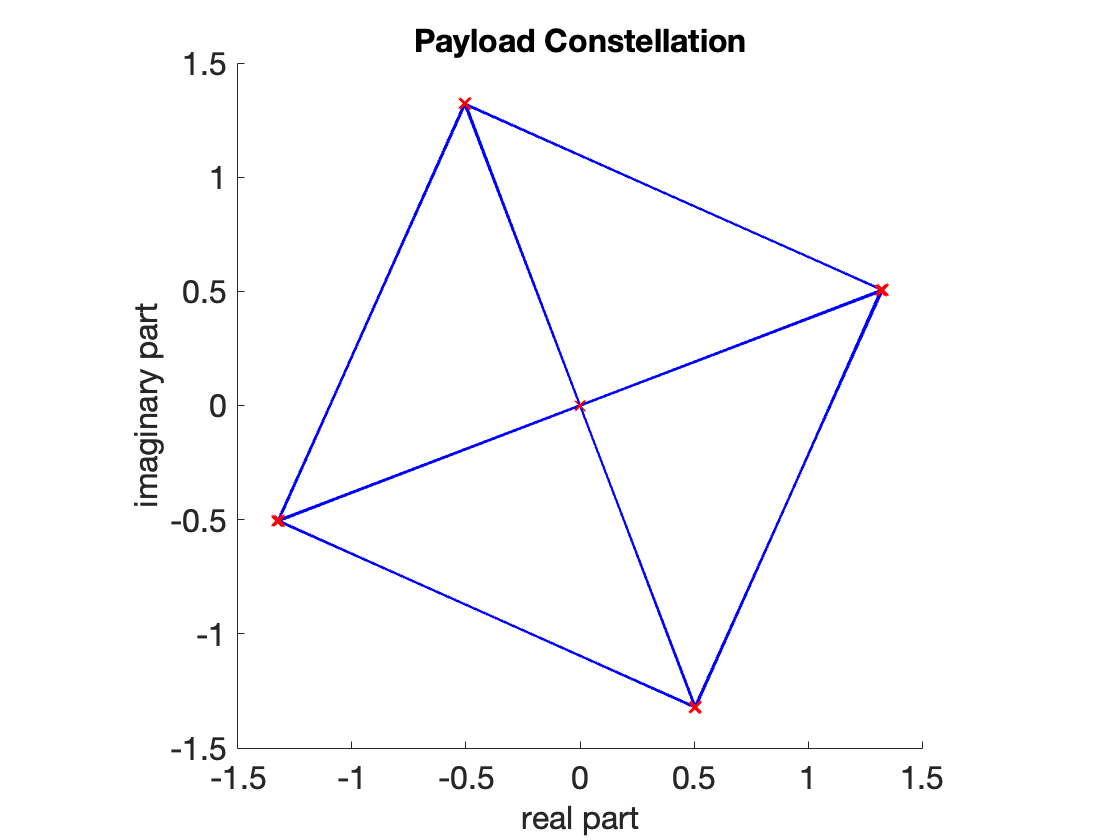
\includegraphics[scale=0.4]{figures/ideal-channel-carrier-phase.png}
    \caption{Ideal Channel xRF1.mat with Carrier Phase Offset}
    \label{fig:phase-rotate}
\end{figure}
\begin{figure}[h!]
    \centering
    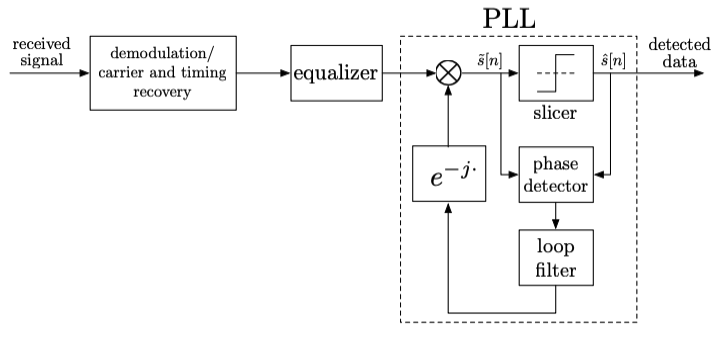
\includegraphics[scale=0.4]{figures/phase_pll.png}
    \caption{Data-Aided Phase PLL}
    \label{fig:phase-pll}
\end{figure}
\begin{figure}[h!]
    \centering
    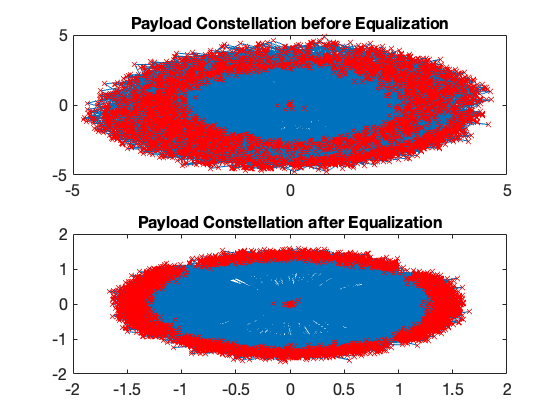
\includegraphics[scale=0.4]{figures/payload_xrf7_before_dd.png}
    \caption{Payload of xRF7.mat Before Decision Directed Carrier Phase Removal}
    \label{fig:before-dd}
\end{figure}
\begin{figure}[h!]
    \centering
    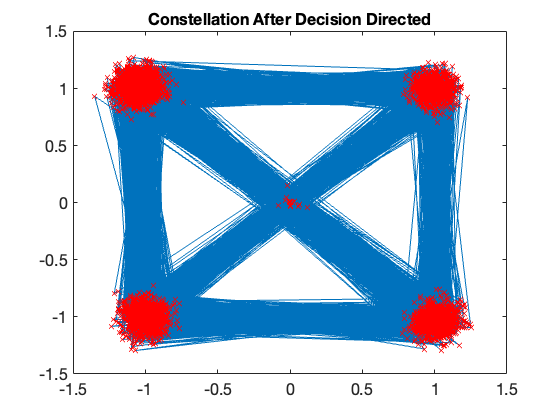
\includegraphics[scale=0.4]{figures/payload_xrf7_after_dd.png}
    \caption{Payload of xRF7.mat After Decision Directed Carrier Phase Removal}
    \label{fig:after-dd}
\end{figure}


\begin{figure}[h!]
    \centering
    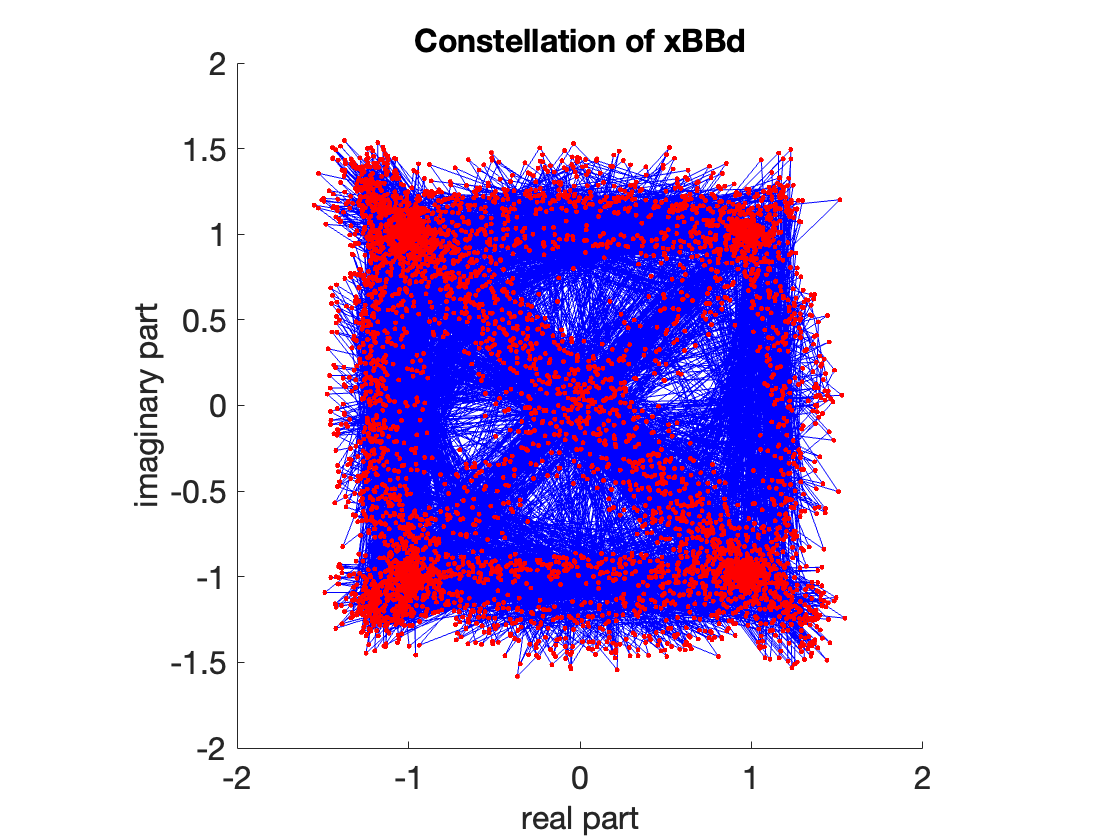
\includegraphics[scale=0.4]{figures/no-timing-phase-corr-xrf9.png}
    \caption{Payload of xRF9.mat No Decision Directed Timing Phase Recovery}
    \label{fig:no-dd}
\end{figure}
\begin{figure}[h!]
    \centering
    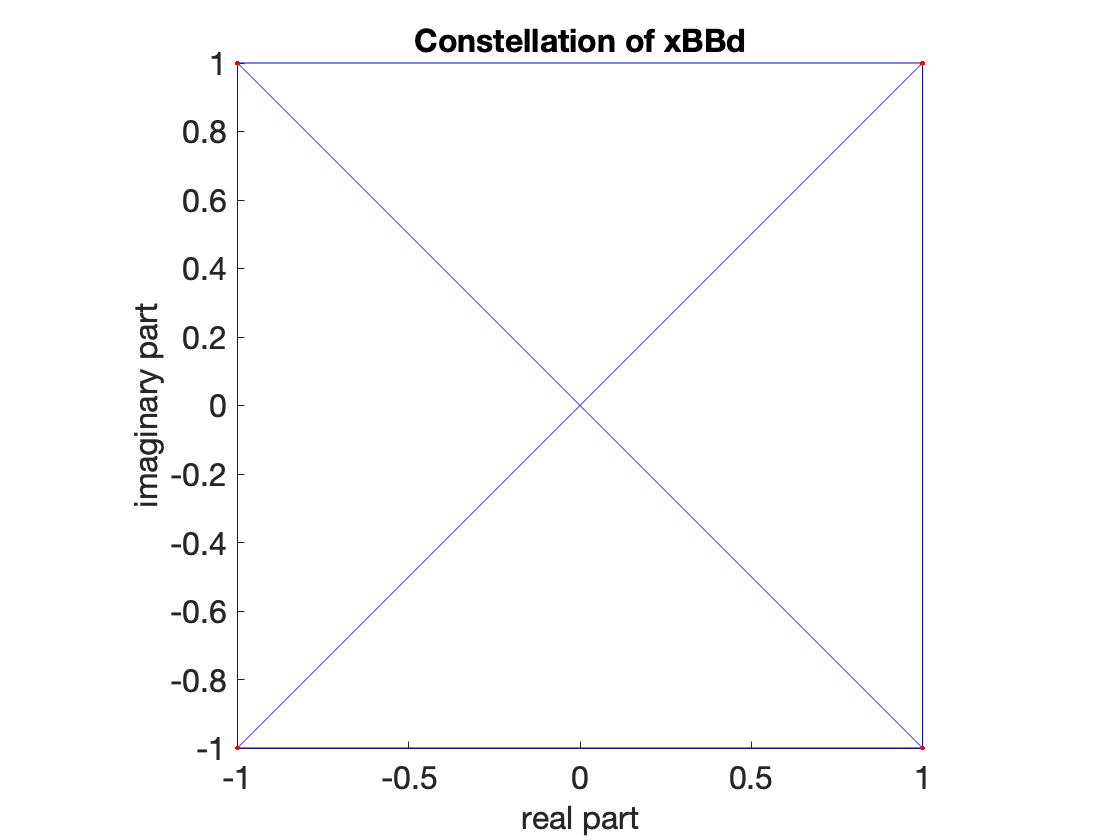
\includegraphics[scale=0.4]{figures/timing-phase-corrected-xrf9.png}
    \caption{Payload of xRF9.mat with Decision Directed Timing Phase Recovery}
    \label{fig:with-dd}
\end{figure}

\begin{figure}[h!]
    \centering
    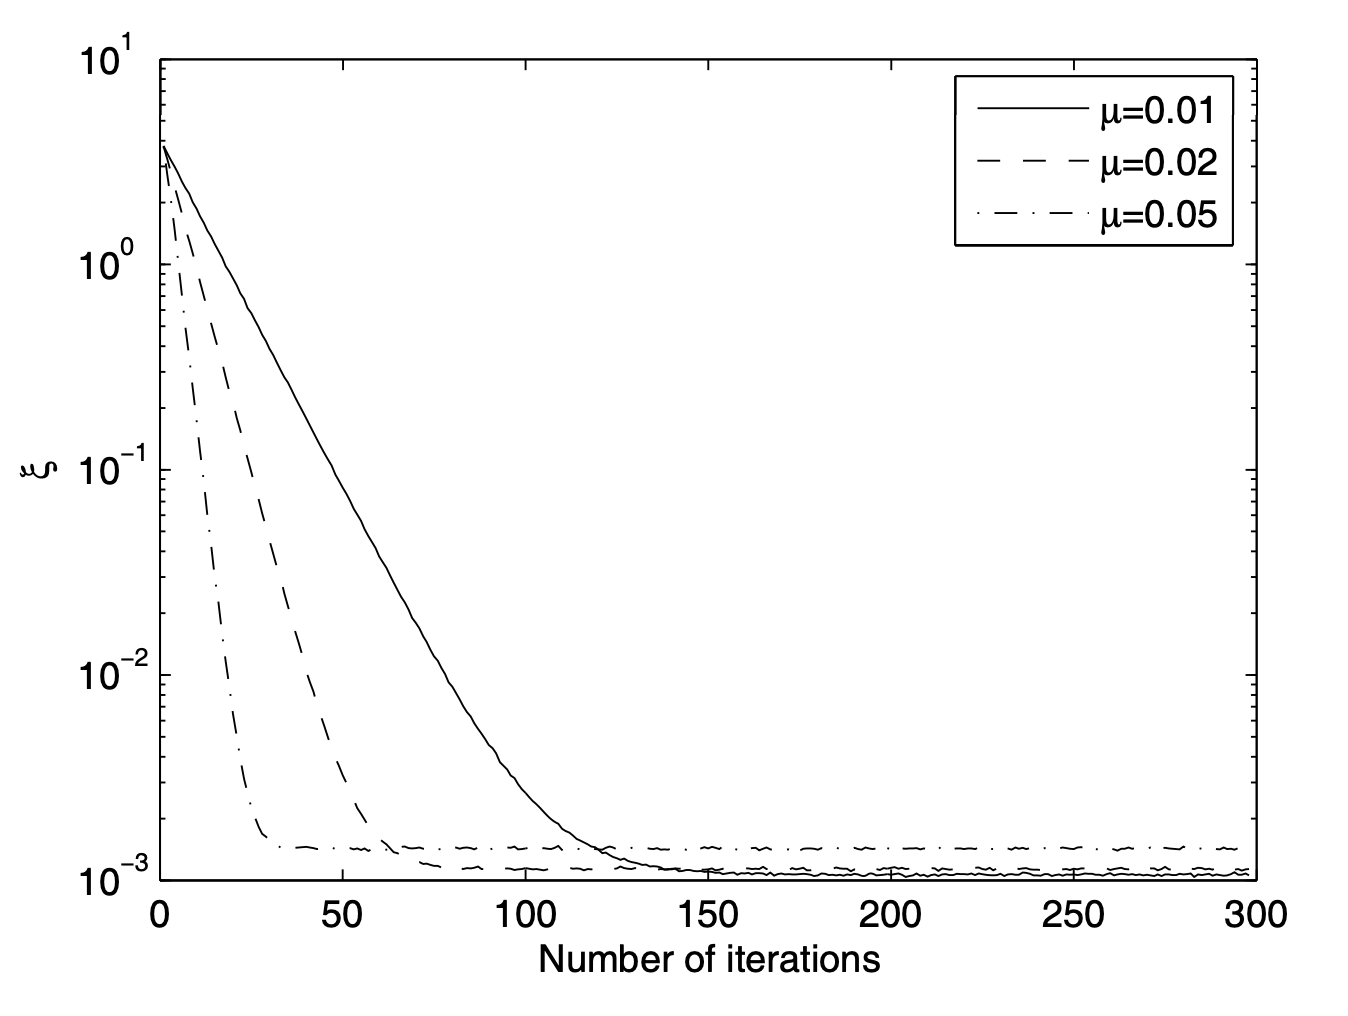
\includegraphics[scale=0.7]{figures/lms-convergence.png}
    \caption{LMS Convergence Rates}
    \label{fig:lms-conv}
\end{figure}
\begin{figure}[h!]
    \centering
    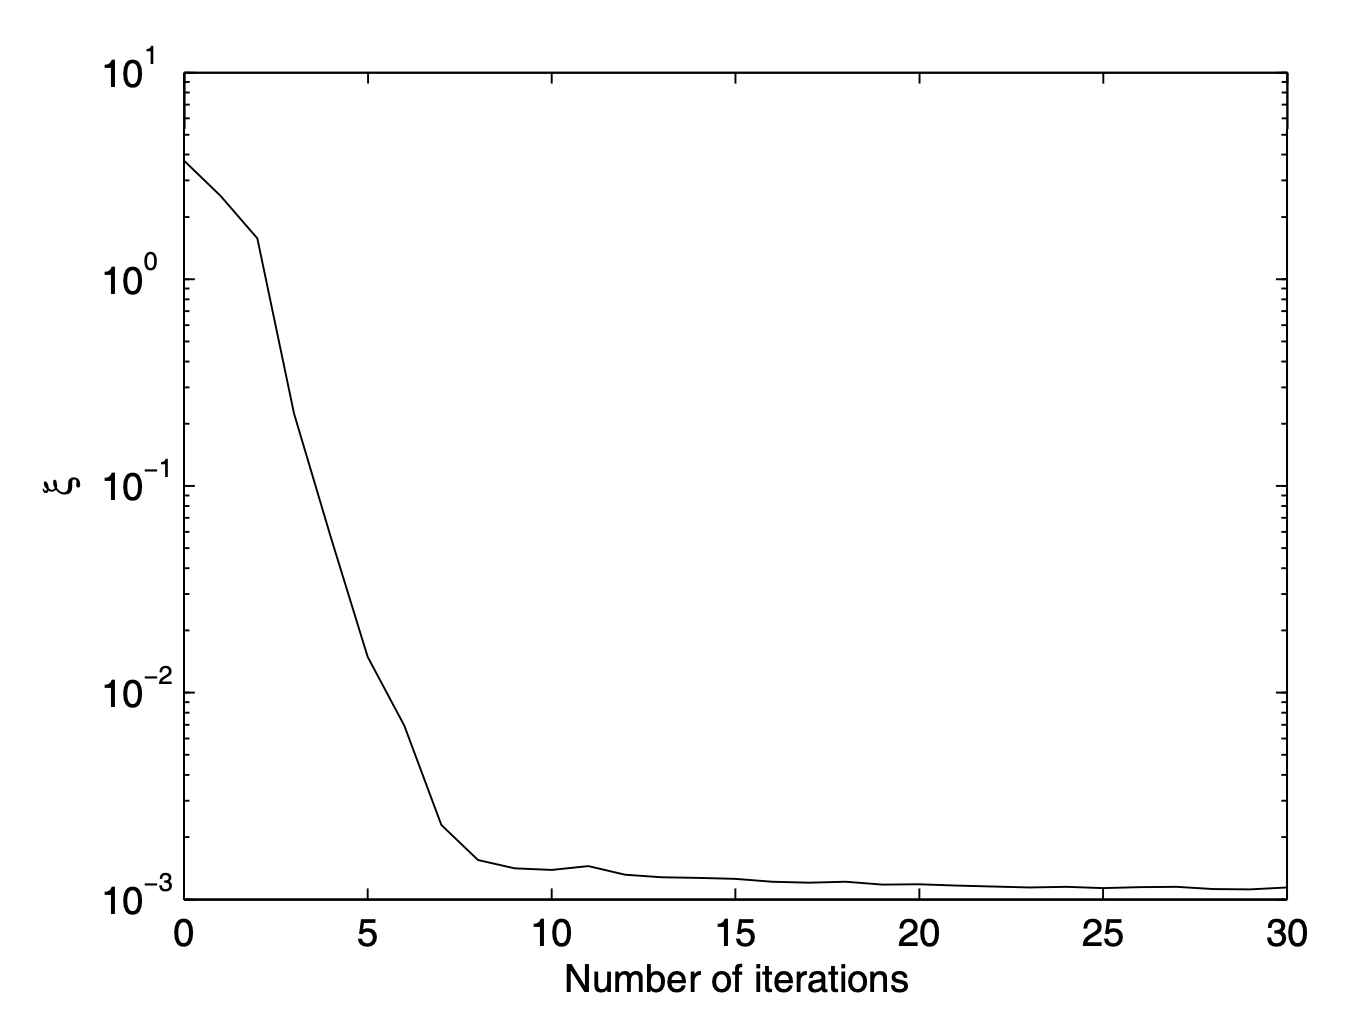
\includegraphics[scale=0.7]{figures/rls-convergence.png}
    \caption{RLS Convergence Rates}
    \label{fig:rls-conv}
\end{figure}

\end{document}